\documentclass[xcolor=dvipsnames,hyperref={pdfpagelabels=false}]{beamer}

\usetheme{Boadilla}

\newcommand{\bi}{\begin{itemize}}
\newcommand{\ei}{\end{itemize}}
\newcommand{\be}{\begin{enumerate}}
\newcommand{\ee}{\end{enumerate}}
\newcommand{\bc}{\begin{center}}
\newcommand{\ec}{\end{center}}
\newcommand{\bd}{\begin{description}}
\newcommand{\ed}{\end{description}}
\newcommand{\I}{\item}
\newcommand{\f}{\frame}
\newcommand{\ft}{\frametitle}

\title{Offline Software Overview}
\subtitle{GlueX Collaboration Meeting}
\author[Mark Ito]{Mark M.\ Ito}
\date{February 21, 2014}
\institute[JLab]{Jefferson Lab}

\begin{document}

\f{\titlepage}

\f{\ft{Other Related Talks}
\bi
\I Software Review (Curtis, Opening Session)
\I Online Data Challenge (David, Online Session)
\I Tracking Improvements (Simon, this session)
\I Offline Data Challenge (Curtis, this session)
\ei
}

\f{
\bi
\I Data Management Plan
  \bi
  \I From the JLab plan summary:
    \bi
    \I Jefferson Lab requires that valuable data...be managed in a way that allows future...researchers to be able to work with the data...this mandate includes the preservation of the data, documentation of the data format...run conditions and calibration databases, and...software used to read and process the data.
    \ei
  \I for the Lab and as a reference for researchers
  \I document hierarchy developed Lab-wide
  \I meeting with Library School folks from CMU
    \bi
    \I same problem as us: funding agencies want to to see this
    \ei
  \ei
\I Data Flow Tools
  \bi
  \I in a nutshell: specify and submit a series of jobs
  \I provide requisite bookkeeping service
  \I SciComp convened the committee; requirements document written
  \I implementation slowed by Lab re-organization
  \I will not be ready for this data challenge
  \ei
\ei
}

\f{
$$
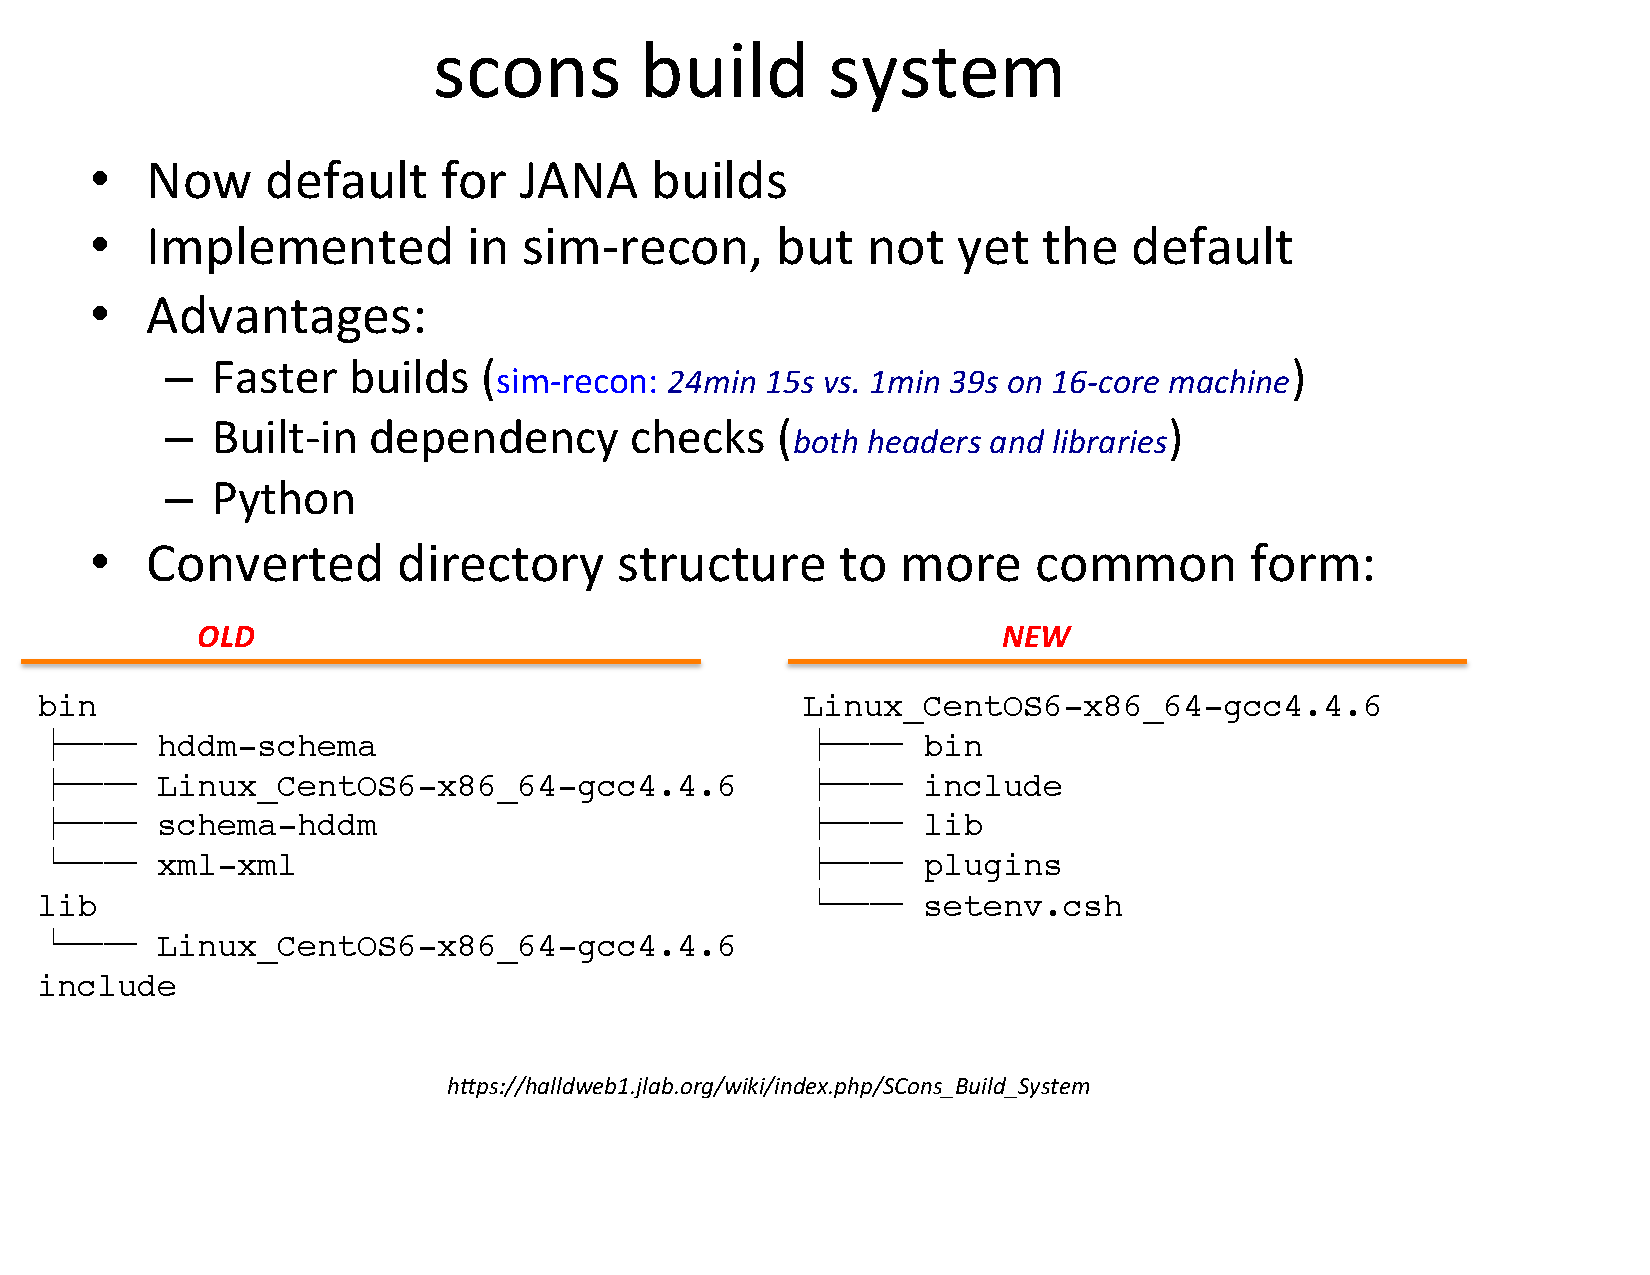
\includegraphics[width=0.9\textwidth]{scons.pdf}
$$
}

\f{$$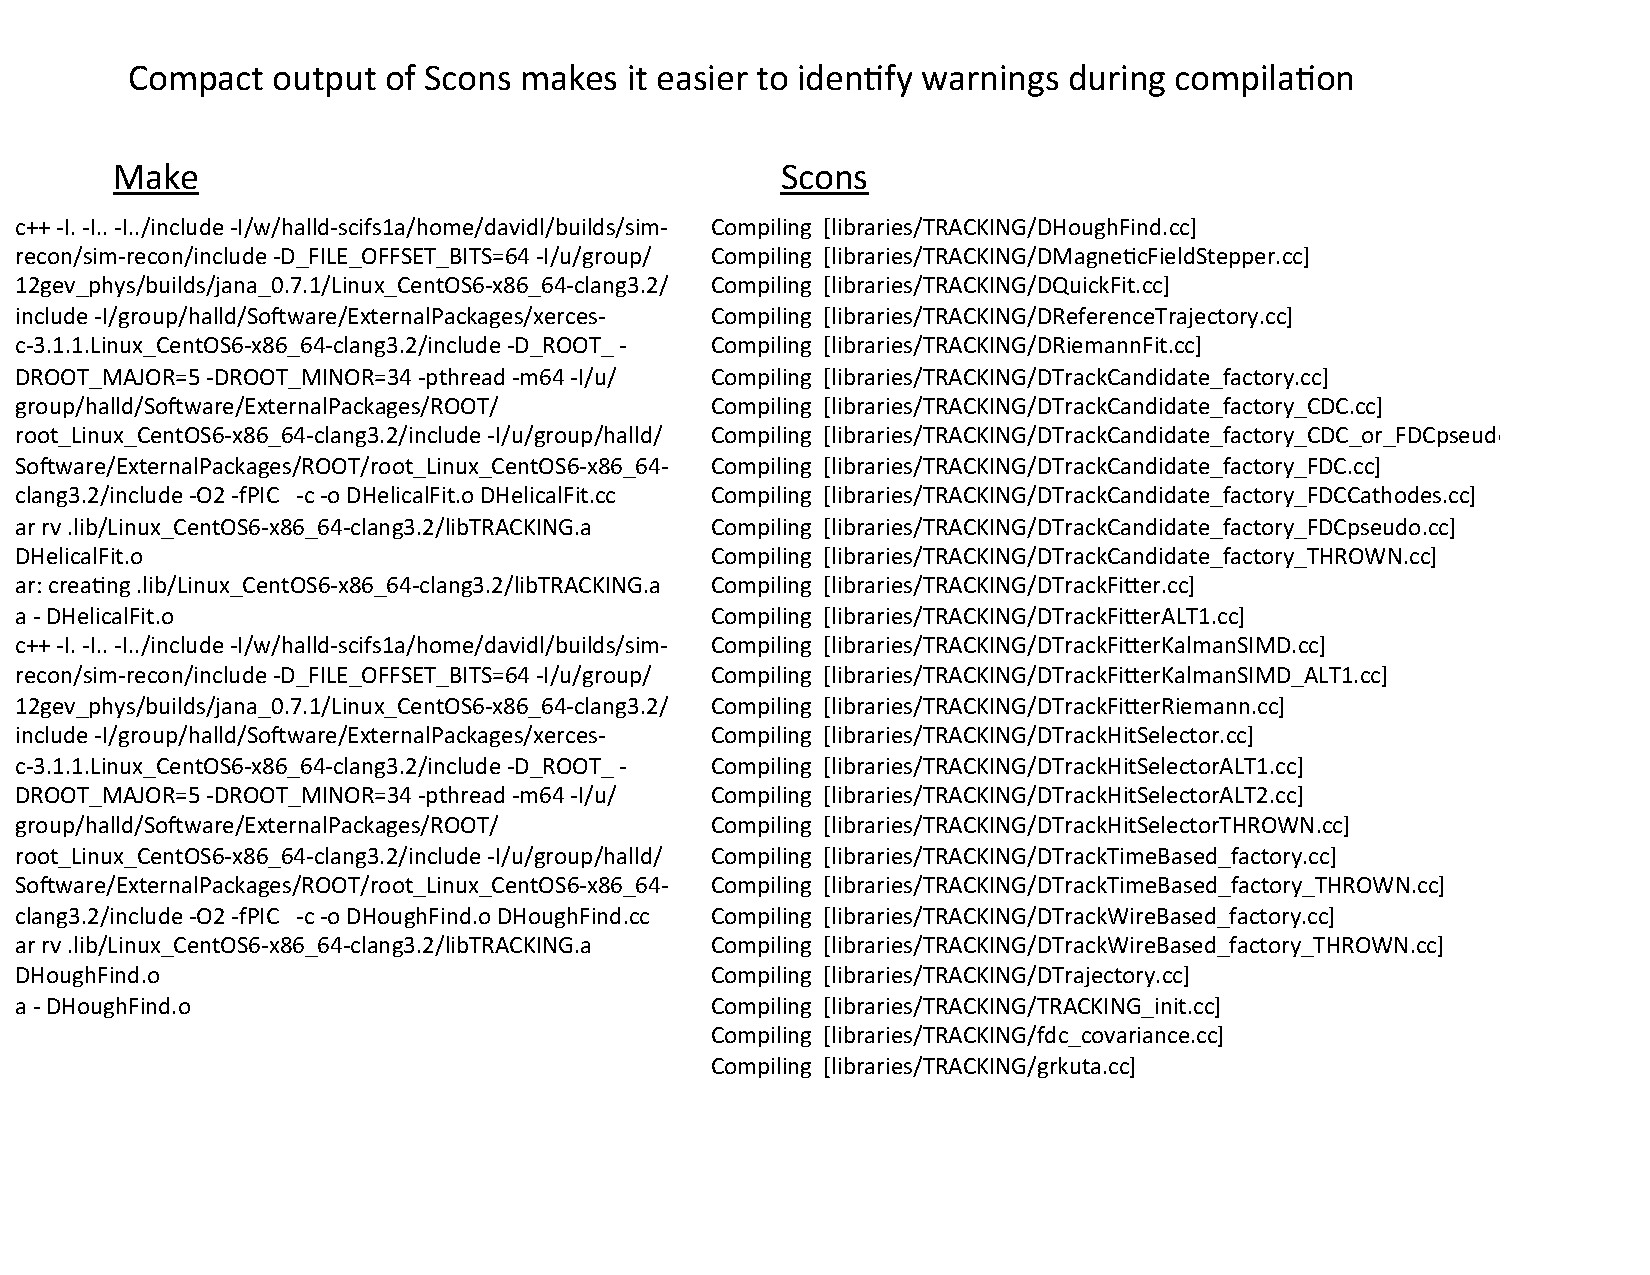
\includegraphics[width=0.9\textwidth]{build_output.pdf}$$}
  
\f{
\bi
\I Monte Carlo Genealogy (MMI)
  \bi
  \I scheme that allows family tree to cross over from bggen to hdgeant
  \ei
\I REST Format and Track Swimming (Paul M.)
  \bi
  \I before: no information on cluster matching to tracks saved
  \I now: matching information kept in REST format
  \ei
\I CCDB (Dmitry)
  \bi
  \I version 0.09 released
    \bi
    \I closes idle MySQL connections
    \I general improvements: help pages, better unit testing, documentation updates, web-site tweaks
    \ei
  \I authentication implemented
  \I plan for Halls A and C to adopt use (B already using it)
  \I SQLite versions of CCDB generated automatically, daily
  \ei
\ei
}

\f{
\bi
\I Splitting up the packages (Paul M., Matt)
  \bi
  \I major categories: simulation, reconstruction, analysis
  \I other stand-alone candidates: HDDM, ``utilities''
  \I addresses some issues with analyzing old data with modern analysis
  \I still in planning stage
  \ei
\I Tagged File System for Event Data (Gagik Gavalian, ODU)
  \bi
  \I Event file distribution
  \I tags: identify relevant files
  \I filters: select out events of interest
  \ei
\I EventStore being explored
  \bi
  \I system for tagging individual events
  \I use one data file for multiple skims
  \I used at CLEO, Matt introduced it to us
  \I Sean in contact with an author
  \ei
\I Time-of-Flight Geometry Changes
  \bi
  \I added half-width counters (Beni, Simon)
  \ei
\ei
}

\f{$$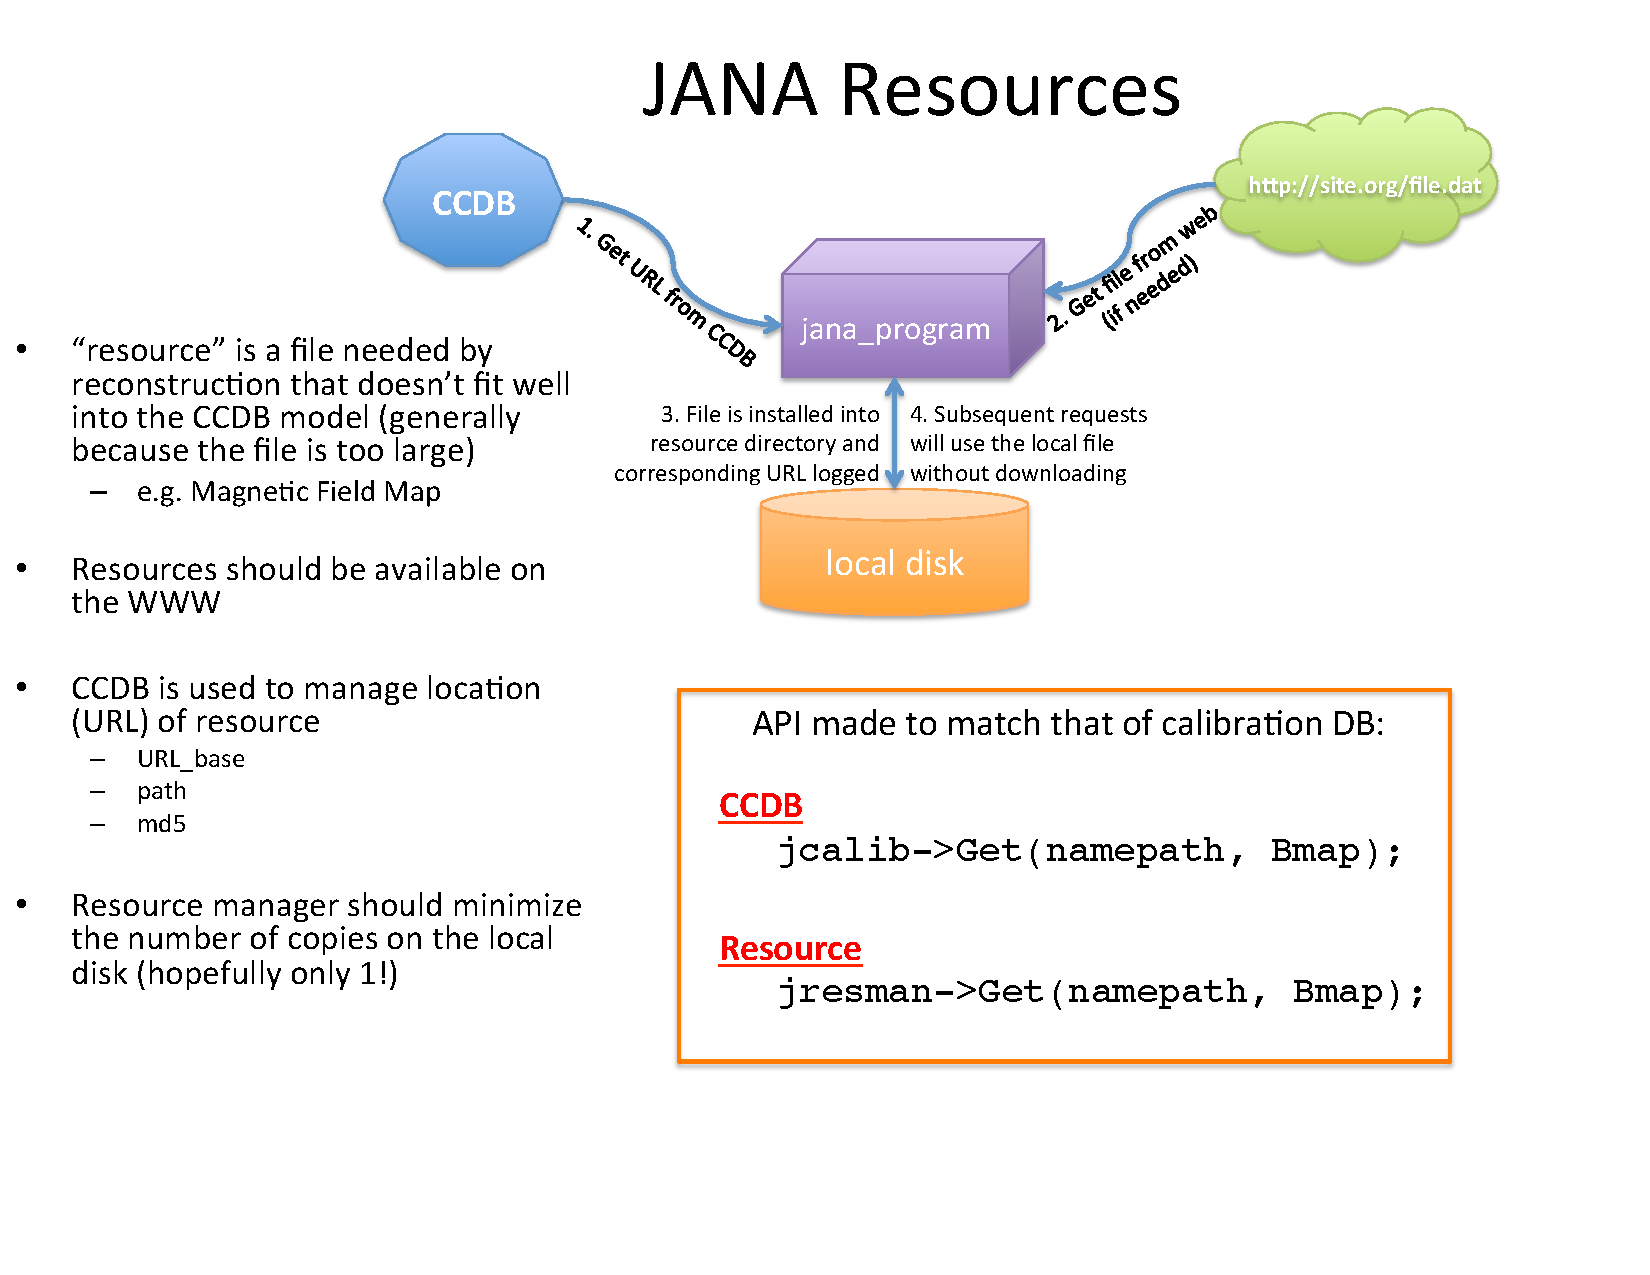
\includegraphics[width=0.9\textwidth]{resources.pdf}$$}

\f{\ft{Geant4}
\bi
\I  progress on geometry
\I  Richard described changes needed last collab. meeting; G4 pickier than G3
\I  changes are done to both; required for apples-to-apples comparison
\I  some side-effects of those changes lingered and needed to be been addressed; done now
\ei
}

\f{$$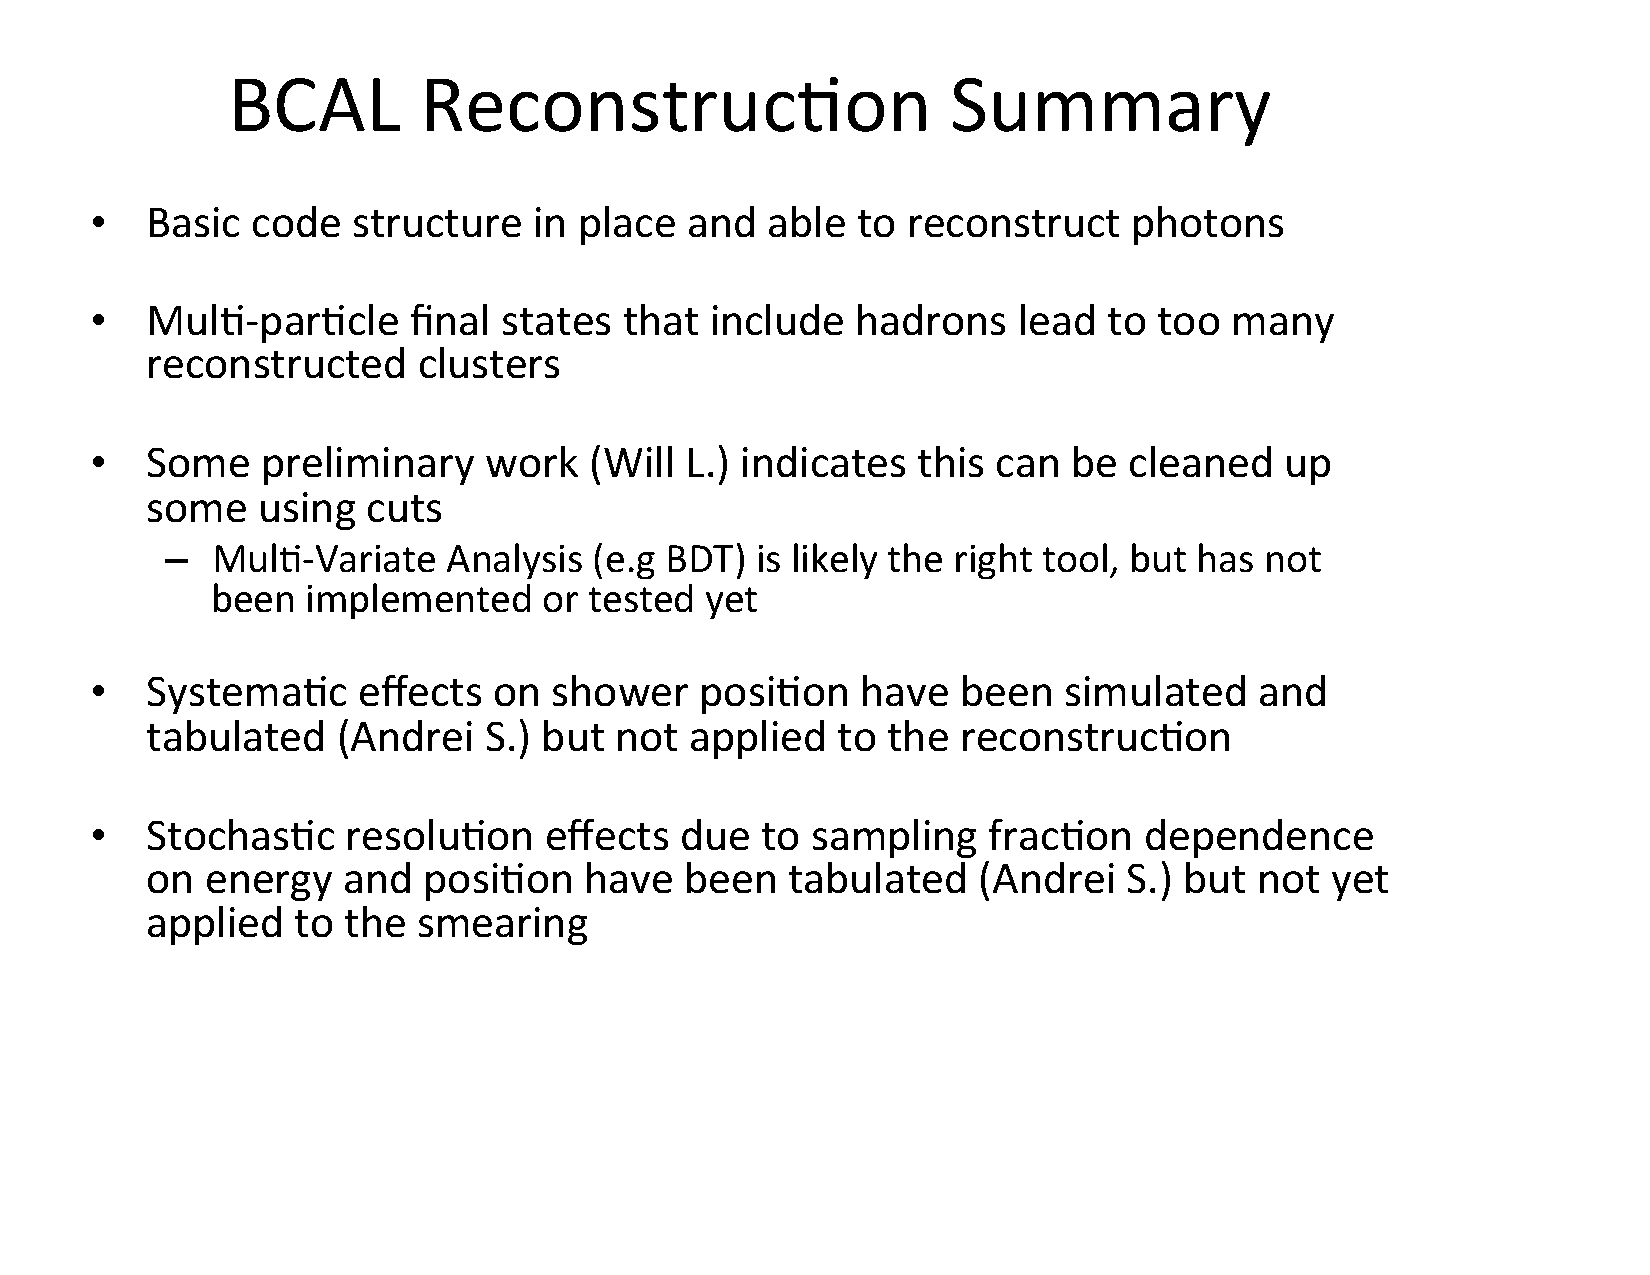
\includegraphics[width=0.9\textwidth]{bcal_recon.pdf}$$}

\f{$$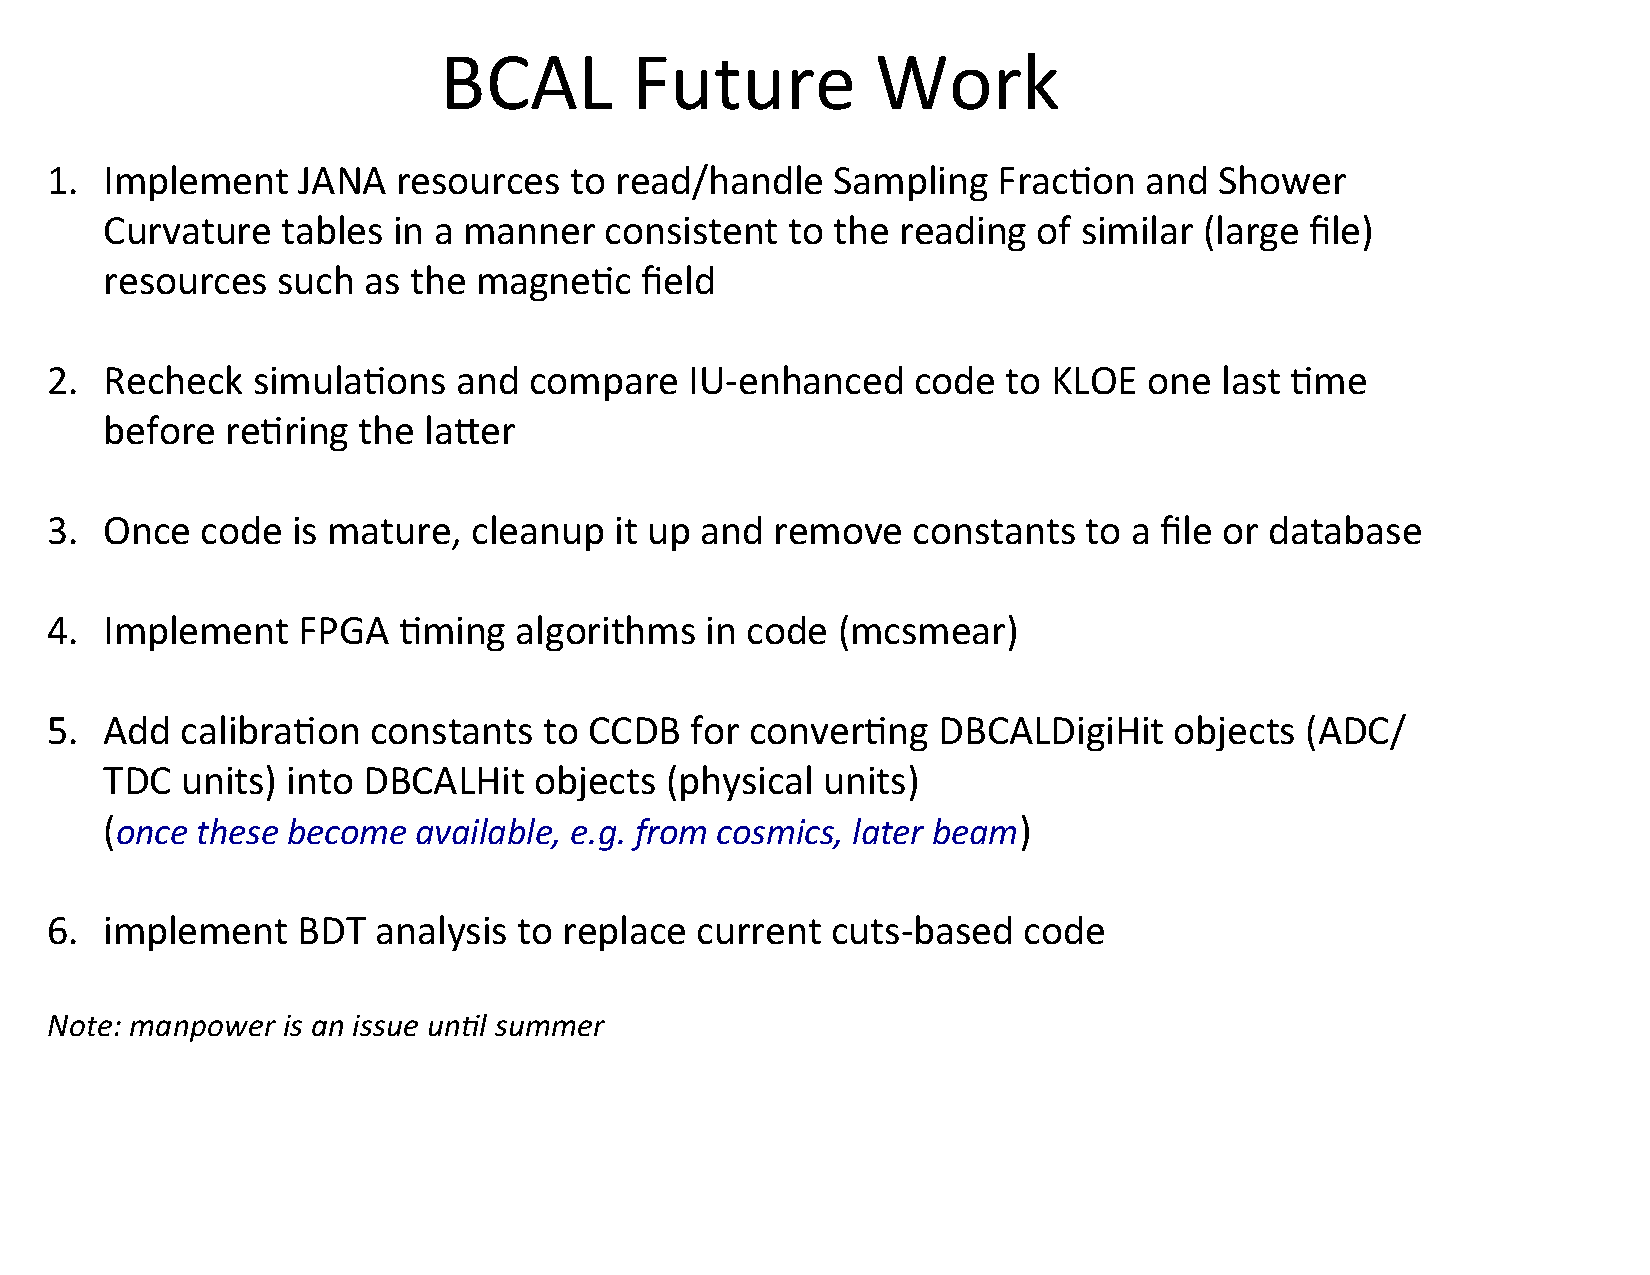
\includegraphics[width=0.9\textwidth]{bcal_future.pdf}$$}

\f{\ft{Conclusions}
\bi
\I Infrastructure is in place for commissioning
  \bi
  \I development driven from online data challenge fills in final pieces, especially ability to reconstruct EVIO-based data
  \I infrastructure needs filling:
    \bi
    \I monitoring histograms
    \I reconstructed quantity monitoring
    \ei
  \ei
\I On the road to smooth, efficient physics analysis
  \bi
  \I AmpTools, Analysis Library, BDT's and other MVA tools
  \ei
\I System improvements still require attention
   \bi
   \I EventStore
   \I Geant4
   \I Meta-data catalog
   \I code profiling
   \I photon reconstruction monitoring
   \I reconstruction algorithms may need review, \`a la BCAL
   \I automated shift scheduler ;-)
   \ei
\ei
}

\end{document}
